\chapter{Μεταβλητότητα των \textlatin{AGN} στις ακτίνες Χ} \label{framework}

%{\color{red}: Υπαρχουν και περιοδικες μεταβολες - Θα ελεγαν "Η εργασια αυτη επικεντρονεται στις μη περιοδικες ματαβολες στην παρατηρουμενη ροη ΑΓΝ. Οι Μεταβολες αυτες  παρατηροθβνταο σε ολα τα μηκη κυματος και θεωρειται μια απο τις ...." οχι μονο των ΑΓΝ αλλα και τον αστρικων μελανων οπων και γανικα ολων των διαδικασιων που περιλαμβανουν προσαυξηση υλης πανω σε ενα συμπαγες αντικειμωνο}


% , while optical continuum variations are thought to be related to instabilities in the more extended, colder and optically thick parts of the same disk. The simplistic assumption is that the X-ray and optical variations will be well correlated. This is true in some but not all objects. A comparison of optical and X-ray light curves in a number of sources shows that in some of these, the optical light curve “leads” the X-ray light curve, whereas in others, one finds the opposite behavior. The multiband light curves of many type-I AGNs indicate variability time scales, and variability amplitudes, that seem to be inversely correlated with source luminosity. This is clearly seen in the X-ray and optical bands, where most such studies have been conducted. There are some indications that the driver of the variability amplitude is the BH mass.\cite{netzer_2013}


%Η μεταβλητότητα στους \textlatin{AGN} τύπου Ι παρατηρείται σε όλα τα μήκη κύματος με τις γρηγορότερες μεταβολές να σημειώνονται στις υψηλότερες ενέργειες. Ματαβολές στις σκληρές ακτίνες Χ έχουνπαρατηρηθεί και σε \textlatin{AGN} τύπου ΙΙ. Η σχέση 
 
Mεταβλητότητα της ενεργειακής ροής και του φάσματος (γραμμικού ή συνεχούς) στους ενεργούς γαλαξιακούς πυρήνες παρατηρείται σε όλα τα μήκη κύματος και θεωρείται μια από τις χαρακτηριστικές ιδιότητες των \textlatin{AGN} \cite{netzer_2013}. Οι μεταβολές αυτές είναι χαρακτηριστικές και των αστρικών μελανών οπών και γενικά όλων των διαδικασιών που περιλαμβάνουν προσαύξηση ύλης σε συμπαγές αντικείμενο.\\
Στην εργασία αυτή θα επικεντρωθούμε στις μη περιοδικές μεταβολές στην παρατηρούμενη ροή \textlatin{AGN} στις μαλακές ακτίνες Χ. Αυτό σημαίνει πως οι πηγές με τις οποίες θα ασχοληθούμε είναι κατά βάση \textlatin{AGN} τύπου Ι. 

Η μεταβλητότητα στους \textlatin{AGN} τύπου Ι παρατηρείται σε όλα τα μήκη κύματος με τις γρηγορότερες μεταβολές να σημειώνονται στις υψηλότερες ενέργειες. Ματαβολές στις σκληρές ακτίνες Χ έχουν παρατηρηθεί και σε \textlatin{AGN} τύπου ΙΙ. Η σχέση του πλάτους ματαβλητότητας και της χρονικής κλίμακας της μεταβλητότητας με την συχνότητα δεν είναι ξεκάθαρη. Οι μεταβλητότητες σε διαφορετικές ενεργειακές ροές πολλές φορές συσχετίζονται και αυτό μας δίνει πληροφορίες για τις φυσικές διαδικασίες που λαμβάνουν χώρα στην κεντρική πηγή ακτινοβολίας. Για παράδειγμα μεταβλητότητα στις ακτίνες Χ έχει παρατηρηθεί να συσχετίζεται με μεταβλητότητα της ίδιας πηγής στο οπτικό \cite{2006ASPC..360..101U} \cite{2006ASPC..360..111G}, ενώ μεταβλητότητα στις ακτίνες Χ έχει παρατηρηθεί να συσχετίζεται με μεταβλητότητα στο υπεριώδες \cite{2005A&A...430..435A}. Οι μεταβολές στις ακτίνες Χ ενδεχομένως οφείλονται σε αστάθειες του στέμματος ή του δίσκου προσαύξησης, ενώ οι μεταβολές στο οπτικό ενδεχομένως οφείλονται σε εκτενή, ψυχρότερα και οπτικά πυκνά τμήματα του δίσκου. Ο συσχετισμός των μεταβολών σε διαφορετικά μήκη κύματος δείχνει πιθανή απορρόφηση και επανεκπομπή του αρχικού σήματος από ύλικό της δομής του ενεργού γαλαξιακού πυρήνα.
%({\color{red}: Γιατι? Τι δειχνει αυτο? πχ παρομοιοι φυσικοι μιχανισμοι κλπ), επιπλεον πιαθνον το ενα μηκος κμματος (οπτικο) να ακολουθει τις ακτινες-Χ οποτε βελπει κανεις την ανταποκριση της υλης στο αρχικο σημα....}.  \\

Πιθανές αιτίες της παρατηρούμενης μεταβλητότητας των \textlatin{AGN} είναι μεταβολές στην διάχυση ενέργειας, μη-αξισυμμετρικές δομές, μετάπτωση κεκλιμένων ροών \cite{Brandt}, ή αλλαγές στον ρυθμό προσαύξησης, εκλάμψεις στον δίσκο προσαύξησης, κίνηση θερμών κηλίδων γύρω από την κεντρική \textlatin{SMBH} και (για μεγάλες χρονικές κλίμακες) κίνηση νεφών υδρογόνου που αποκρύπτουν την κεντρική πηγή \cite{2004astro.ph..9151H}.

%({\color{red}: Δεν εχεις εξηγησει τι ειναι \textlatin{PSD}. Επιπλεον γιατι εχωριστο κεφαλαιο για τις ακτινες-Χ. Ισως απλα να εξηγησεις οτι οι ακτινες-Χ παραγονται σε περιοχες πολυ κοντα απο τη μαυρη τρυπα και συνεπως παραεχουν πληροφοειες για την φυσικη της προσασυξησης υλης. για τις διαστασεις της περιχοης εκπμπης. Επιπλεον οι ακτινες-Χ εχουν το καλο οτι αστρικες διαδικασιες παραγουν σχεδον καθολου ακτινοβολια στις ακτινες-Χ. Σε αντιθεση στο οπτικο/υπερυθρο ο γαλαξιας εχειο σημαντικη συνεισφορα η ακομα και υπερεχει (δες πχ https://ui.adsabs.harvard.edu/abs/2015A\%26ARv..23....1B/abstract) και συνεπως μελεταει κανεισ την μετβαλητηοτα λογω της διαδικασοαιας προσαυξησης  και δεν}).

\section{Φασματική πυκνότητα ενεργειακής ισχύος(\textlatin{PSD})}

%{\color{red}: not only at X-rays at any wavelength Για τη μελετη της μεταβλητοτας απαιτουνται παρατηρησεις σε....}
Για την μελέτη μεταβλητότητας αστρονομικών πηγών σε οποιαδήποτε μήκη κύματος χρησιμοποιούμε καμπύλες φωτός (αλλιώς χρονοσειρές), δηλαδή πεπερασμένες σειρές $x(t_i)$ από μετρήσεις ροών $x_i$ με $Ν$ το πλήθος διακριτά σημεία που μετρήθηκαν σε χρόνους $t_i$ me $i=1,2,...,N$. Στα όργανα μέτρησης ακτίνων Χ έχουμε καταγραφές φωτονίων σε διακριτά χρονικά διαστήματα $(t_i , t_{i+1})$\cite{Grant2019}.\\
Η \textlatin{PSD} είναι ένας τρόπος να απεικονίσουμε την μεταβλητότητα της ισχύος ενός σήματος συναρτήσει της χρονικής συχνότητας \textlatin{Fourier} και εκτιμάται υπολογίζοντας το περιοδόγραμμα \cite{Vaughan2}.
Το περιοδόγραμμα είναι μία διακριτή συνάρτηση ισχύος συναρτήσει χρονικής συχνότητας $ P (f_j)$ η οποία εκτιμά την συνεχή \textlatin{PSD} $\mathcal{P}(f)$ (η οποία στις χρονοσειρές \textlatin{AGN} σε μια πρώτη προσέγγιση συμπεριφέρεται ως $ \mathcal{P}(f) \propto f^{-\alpha}$, με το $\alpha \approx 2$ κατά μέσο όρο). Αν τα δεδομένα (η καμπύλη φωτός $x(t_i)$) ακολουθούν ομοιόμορφη δειγματοληψία (με περίοδο συλλογής $\Delta T$), το περιοδόγραμμα είναι ο διακριτός μετασχηματισμός \textlatin{Fourier} της καμπύλης φωτός $X(f_j)$, κανονικοποιημένος κατά $\sqrt{\frac{\Delta T}{N}}$ ώστε τα πλάτη να είναι ανεξάρτητα της συχνότητας δειγματοληψίας και του μήκους της καμπύλης φωτός. Το αποτέλεσμα του κανονικοποιημένου αυτού μετασχηματισμού είναι μιγαδική διακριτή συνάρτηση $X(f_j)$ με $Ν/2$ ισαπέχουσες συχνότητες η οποία, αφού τετραγωνιστεί με την μιγαδική συζυγή της, με κατάλληλη κανονικοποίηση αποτελεί το περιοδόγραμμα\cite{Vaughan2}:
\begin{equation} P(f_j) = \frac{2}{\overline{x}^2} |X(f_j)|^2  \end{equation}

\subsection{Θόρυβος \textlatin{Poisson}}
Αν οι χρονοσειρές είναι σήμα καταμέτρησης φωτονίων (και όχι ροές), όπως συμβαίνει στην αστρονομία ακτίνων Χ, και ομαδοποιηθούν σε χρονικά διαστήματα $\Delta T$, τότε η επίδραση θορύβου \textlatin{Poisson} έχει ώς αποτέλεσμα την πρόσθεση μιας σχεδόν σταθερής ποσότητας ισχύος στο περιοδόγραμμα σε όλες τις συχνότητες \cite{2003MNRAS.345.1271V} όπως βλέπουμε και στο σχήμα \ref{fig:LCandPSD}.

\begin{figure*}%
    \centering
    \subfloat{{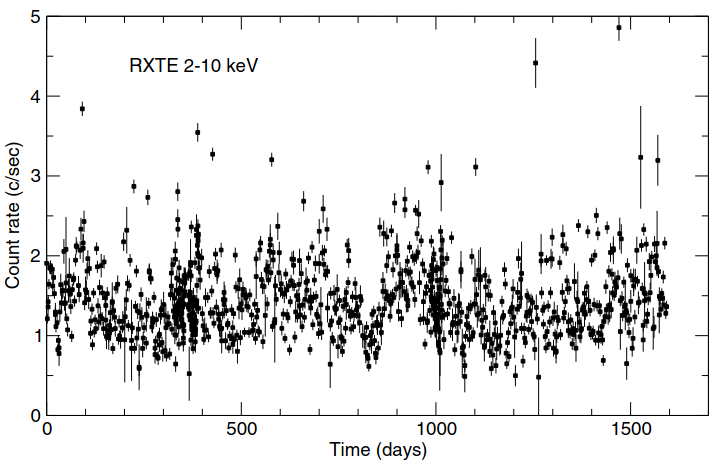
\includegraphics[width=0.42\linewidth]{Figures/PapadakisLC.png} }}%
    \qquad
    \subfloat{{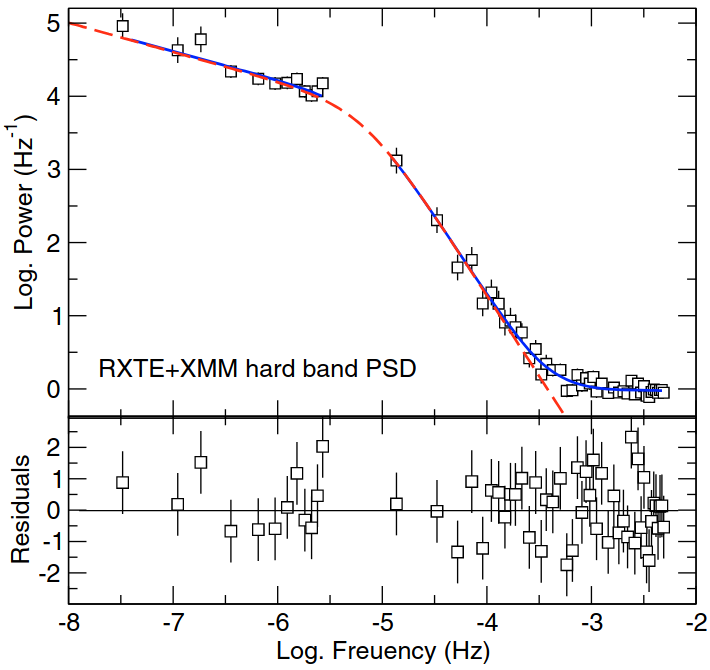
\includegraphics[width=0.5\linewidth]{Figures/PapadakisPSD.png} }}%
     \caption{Αριστερά: Δείγμα καμπύλης φωτός ακτίνων Χ ενεργού γαλαξιακού πυρήνα. Δεξιά: Ο διακριτός μετασχηματισμός \textlatin{Fourier} της καμπύλης φωτός- κατάλληλα κανονικοποιημένος- μας δείνει το περιοδόγραμμα (διακριτά σημεία) το οποίο προσεγγίζει την \textlatin{PSD} (κόκκινη διακεκομένη γραμμή) ενώ παρατηρούμε και το σταθερό υπόβαθρο θορύβου \textlatin{Poisson} (φαίνεται καθαρά στην μπλέ συνεχή καμπύλη ως σταθερά στις μεγάλες συχνότητες)\cite{2010A&A...518A..28P}.} \label{fig:LCandPSD}
\end{figure*}

\subsection{Μέσος όρος και ομαλοποίηση περιοδογράμματος}

Το περιοδόγραμμα σε μια δεδομένη συχνότητα $P(f_0)$ διασπείρεται γύρω από την \textlatin{PSD} $\mathcal{P}(f_0)$ ακολουθώντας μια κατανομή $\chi^2$ δύο βαθμών ελευθερίας:
\begin{equation}
    P(f_0) = \mathcal{P}(f_0)\dfrac{\chi^2_2}{2}
\end{equation}
και είναι ασύμφωνο με την \textlatin{PSD}, καθώς η διασπορά στο περιοδόγραμμα δεν μειώνεται αυξάνοντας το πλήθος των σημείων στην καμπύλη φωτός. Προκειμένου να περιοριστεί η διασπορά παίρνουμε τον μέσο όρο του περιοδογράμματος (είτε ομαδοποιώντας (\textlatin{bin}) τις συχνότητες είτε παίρνοντας μέσο όρο τμημάτων δεδομένων) με αποτέλεσμα ο μέσος όρος αυτός του περιοδογράμματος να συμφωνεί με την \textlatin{PSD}\cite{2003MNRAS.345.1271V}.
Για να περιοριστεί η διασπορά το περιοδόραμα υποβάλεται και σε <<vομαλοποίηση>> (\textlatin{smoothing}), δηλαδή υπολογίζεται η ενεργειακή πυκνότητα σε μία συχνότητα ως μέσος όρος με ειδικό βάρος (\textlatin{weighted average}) των γειτονικών τιμών του περιοδογράμματος. Η συνάρτηση ειδικού βάρους $W$ λέγεται <<φασματικό παράθυρο>> \cite{1993MNRAS.261..612P}.

\subsection{Γενική μορφή \textlatin{PSD} ενεργών γαλαξιών}
Για κοντινά \textlatin{AGN} η προσαρμογή (\textlatin{fitting}) φασματικών δεδομένων  έχει ως αποτέλεσμα την μοντελοποίηση των \textlatin{PSD} ενεργών γαλαξιών είτε ώς νόμο δύναμης ($\mathcal{P}(f)\propto f^{-\alpha}$), είτε ώς κυρτωμένο νόμο δύναμης με συχνότητα ανακοπής $f_b$\cite{2017MNRAS.471.4398P}.
 
\section{Ολοκλήρωμα της ενεργειακής ισχύος}

Το αναλυτικό ολοκλήρωμα της (συνεχούς) συνάρτησης της \textlatin{PSD} $\mathcal{P}(f)$ μεταξύ δύο συχνοτήτων ($f_1$ και $f_2$) είναι ένα μέτρο της μέσης φασματικής ισχύος του σήματος και μας δίνει την συνεισφορά των διακυμάνσεων μεταξύ των αντίστοιχων κλιμάκων χρόνου ($1/f_1$ και $1/f_2$) στην αναμενόμενη τιμή της (<<πραγματικής>>) διακύμανσης\cite{2003MNRAS.345.1271V}:
\begin{equation} <\mathcal{S}^2> = \int_{f_1}^{f_2} \mathcal{P}(f)df  \label{eq:integratedPSD} \end{equation}
Αντίστοιχα, για διακριτή χρονοσειρά, το <<vολοκληρωμένο>> περιοδόγραμμα μας δίνει την παρατηρούμενη διακύμανση για την συλλογή δεδομένων\cite{2003MNRAS.345.1271V}: 
\begin{equation} S^2 = \sum_{j=1}^{N/2} P(f_j)\Delta f \label{eq:integratedperiodogram} \end{equation}
Όπου $\Delta f$ είναι η διακριτότητα στις συχνότητες του διακριτού μετασχηματισμού \textlatin{Fourier} ($\Delta f = \frac{1}{N\cdot \Delta T}$). \\
Η συνολίκή διακύμανση μιας πραγματικής καμπύλης φωτός είναι το ολοκλήρωμα του περιοδογράμματος $P(f_j)$ από την χαμηλότερη συχνότητα του διακριτού μετασχηματισμού \textlatin{Fourier} έως την υψηλότερη \cite{2003MNRAS.345.1271V}. Ο διακριτός μετασχηματισμός \textlatin{Fourier} υπολογίζεται σε $Ν/2$ το πλήθος ισοκατανεμημένες συχνότητες $f_j = \frac{j}{N\cdot \Delta T}$ me $(j = 1, 2, . . . , N/2)$, έτσι η χαμηλότερη συχνότητα του μετασχηματισμού είναι $f_1 = \frac{1}{N \cdot \Delta T}$ και η υψηλότερη $f_{Nyq} = \frac{1}{2  \Delta T}$ \cite{Vaughan2}.\\
H διακύμανση για την καμπύλη φωτός (χρονοσειρά) που συλλέγουμε για μια πηγή είναι (υπολογισμένη απόστοιχεία φωτομετρίας της καμπύλης φωτός): 
\begin{equation} S^2 = \frac{1}{N-1} \sum_{i=1}^{N} (x_i-\overline{x})^2 \label{eq:fluxvariance}\end{equation}
Όπου $\overline{x}$ είναι ο αριθμητικός μέσος των $x_i$ σημείων της χρονοσειράς ροής (καμπύλης φωτός). Αυτή διαφέρει από μια συλλογή δεδομένων (παρατήρηση) σε άλλη συλλογή δεδομένων της ίδιας πηγής, αφού το περιοδόγραμμα είναι μια αναπαράσταση της πραγματικής \textlatin{PSD} που εξαρτάται από την υλοποίηση της συλλογής δεδομένων (χρονοσειρά).\\
Στο όριο μεγάλου $Ν$ αυτές οι δύο προσεγγίσεις διακύμανσης (ολοκλήρωμα περιοδογράμματος \ref{eq:integratedperiodogram} και διακύμανση ροής \ref{eq:fluxvariance}) είναι ταυτοτικές. Η κανονικοποιημένη διακύμανση είναι $\frac{S^2}{\overline{x}^2}$ \cite{2003MNRAS.345.1271V}.

%%===================================%
%%===================================%
%%===================================%
\section{H \textlatin{NXSV} ως μέγεθος εκτίμησης μεταβλητότητας}

\subsection{Κανονικοποιημένη πλεονάζουσα διακύμανση(\textlatin{NXSV}) $\sigma_{rms}^2$}
 
Η ανάλυση των \textlatin{PSD} (μέσω περιοδογράμματος) είναι ένα εξαιρετικό εργαλείο για να εξεταστούν και να χαρακτηριστούν οι ιδιότητες της μεταβλητότητας των \textlatin{AGN}, ωστόσο, για να αποδόσει πλήρως απαιτεί μακροσκελείς αδιάκοπες παρατηρήσεις με διεξαγωγή παρακολουθήσεων ειδικών προδιαγραφών. Τέτοιου είδους παρατηρήσεις δεν διατίθενται για μεγάλο αριθμό πηγών, όμως υπάρχουν βραχείες παρατηρήσεις στις ακτίνες Χ με αρκετά μεγάλο λόγο σήματος προς θόρυβο (\textlatin{S/N}) πληθώρας \textlatin{AGN}- ιδίως για το παρατηρητήριο \textlatin{XMM-Newton}, λόγω της μεγάλης ευαισθησίας του και του εύρους των ενεργειών που καλύπτει. \\
Ένα χρήσιμο και πρακτικό εργαλείο για την ανάλυση ελλειπών δεδομένων είναι η πλεονάζουσα κανονικοποιημένη διακύμανση(\textlatin{NXSV}) $\sigma_{rms}$:
\begin{equation} \sigma^2_{rms} = \frac{1}{N \cdot {\overline{x}}^2 }   \sum_{i=1}^{N}  [ (x_i -\overline x)^2  - x_{err, i}^2]  \label{eq:NXSVformula}\end{equation}
Όπου $\overline x$ η μέση ροή στην χρονοσειρά $x_i$ ροών με $Ν$ το πλήθος σημεία, ενώ $x_{err, i}$ είναι η αβεβαιότητα στην μέτρηση ροής $x_i$. \\
Ο όρος $ \frac{1}{N }   \sum_{i=1}^{N}   (x_i -\overline x)^2  $ αναπαριστά την διακύμανση του σήματος, ο όρος $ \frac{1}{N }   \sum_{i=1}^{N}  x_{err, i}^2 $ αναπαριστά την διακύμανση του στατιστικού σφάλματος (θορύβου), η διαφορά των δύο είναι η πλεονάζουσα διακύμανση, και κανονικοποιώντας με τον παράγοντα $ \frac{1}{{\overline{x}}^2 }$ προκύπτει η κανονικοποιημένη πλεονάζουσα διακύμανση.\\
Η \textlatin{NXSV} είναι η μέση τετραγωνική απόκλιση που μετράμε στην καμπύλη φωτός διορθωμένη κατά το στατιστικό σφάλμα και είναι ένα μέγεθος που ποσοτικοποιεί την διακύμανση, αποτελεί δηλαδή ένα <<πλάτος>> μεταβλητότητας\cite{2004ApJ...611...93P}.\\
Σε αντιπαραβολή με την ολοκλήρωση περιοδογράμματος (\ref{eq:integratedperiodogram} ) που προσεγγίζει το ολοκλήρωμα της \textlatin{PSD} (\ref{eq:integratedPSD}), η \textlatin{NXSV} είναι το ολοκλήρωμα της \textlatin{PSD} από μία ελάχιστη κλίμακα χρόνου (μέγιστη συχνότητα) μέχρι μία μέγιστη κλίμακα χρόνου (ελάχιστη συχνότητα), η μεταβολή στην ροή επιφέρει μεταβολή στο σχήμα της \textlatin{PSD} ή στην συχνότητα αποκοπής (για κυρτωμένη \textlatin{PSD}), έτσι, αφού το φάσμα αλλάζει, με την ολοκλήρωση καταγράφουμε το πλάτος της μεταβλητότητας.\\  
Η \textlatin{NXSV} δεν προσφέρει τόση πληροφορία όσο η φασματική ανάλυση των \textlatin{PSD}, αλλά μπορεί να χρησιμοποιηθεί για να ελέγξει ή να επιβεβεώσει αποτελέσματα από φασματική ανάλυση μεμονωμένων \textlatin{AGN} σε μεγάλους πληθυσμούς καθώς και για να ελέγξει τον συσχετισμό ύπαρξης μεταβλητότητας και πλάτους μεταβλητότητας με άλλες φυσικές παραμέτρους των \textlatin{AGN}\cite{2012A&A...542A..83P}.

%%===================================%

\subsection{Αβεβαιότητα και μεροληψία στην \textlatin{NXSV}}

\subsubsection*{Αβεβαιότητα}
Η \textlatin{NXSV}, όπως ορίστηκε στην εξίσωση \ref{eq:NXSVformula}, εκτιμά την εγγενή μεταβλητότητα της καμπύλης φωτός κατά μέγιστη πιθανότητα \textlatin{(maximum likelihood- ML)} μόνο στην περίπτωση που έχουμε όμοια, κανονικά κατανεμημένα σφάλματα στις μετρήσεις της χρονοσειράς. Αν αυτό δεν συμβαίνει, τότε δεν υπάρχει αναλυτικός τρόπος μέγιστης πιθανότητας \textlatin{(ML)} που να εκτιμά την εγγενή μεταβλητότητα και απαιτείται αριθμητική προσέγιση\cite{2017MNRAS.471.4398P}. Ωστόσο, πρακτικά, οι δύο αυτοί τρόποι (αναλυτική $\sigma_{rms}^2$ για ίδια κανονικά σφάλαματα και αριθμητική $\sigma_{ML}^2$ για ανομοιόμορφα σφάλματα) για ρεαλιστικές καμπύλες φωτός με <<vαραιές>> καταγραφές δεδομένων δίνουν όμοια αποτελέσματα\cite{2013ApJ...771....9A}. Αυτό είναι αναμενόμενο, καθώς η αβεβαιότητα που οφείλεται σε στοχαστικό θόρυβο \textlatin{(red noise)} στην καμπύλη φωτός είναι πολύ μεγαλύτερη της αβεβαιότητας που οφείλεται στην προσέγγιση αναλυτικής λύσης $\sigma_{rms}^2$.\\

%The datasets considered thus far have been ideal, in the sense that they are free from flux uncertainties. In real life, however, a lightcurve xi will have finite uncertainties σerr,i due to measurement errors (such as Poisson noise in the case of an X-ray photon counting signal). These uncertainties on the individual flux measurements will contribute an additional variance. This leads to the use of the ‘excess variance’ (Nandra et al. 1997; Edelson et al. 2002) as an estimator of the intrinsic source variance. This is the variance after subtracting the contribution expected from measurement errors. --------------------\\ The normalised excess variance is given by σNXS2= σXS2/x̄ 2 and the fractional root mean square (rms) variability amplitude (Fvar ; Edelson, Pike & Krolik 1990; Rodriguez-Pascual et al. 1997) is thesquare root of this, i.e. \cite{2003MNRAS.345.1271V} 

% An empirical estimate of the mean and standard deviation of the variance can be made given M non-overlapping data segments The advantage of the above method is that it requires no assumption about the shape of the PSD, The drawback is that it requires asubstantial amount of data to produce a single, robust variance estimate. An alternative approach is to estimate the standard deviationof the variances Si based on simulations. Given an assumed shape for the PSD it is possible to calculate the distribution of variances expected for a stationary process..  the distribution depends on the slope of the PSD. The distribution becomes more normal at flatter slopes and more asymmetric at steep slopes. \cite{2003MNRAS.345.1271V}  

%the uncertainty in the variance estimate caused by Poisson noise.  the error on σNXS2 decreases as the S/N in the light curve is increased according to: ----- this only accounts for the effect of flux measurement errors (such as Poisson noise) in a given light curve \cite{2003MNRAS.345.1271V} 


%The bias certainly depends on the PSD slope. For the continuous sampling case, b is always smaller than 1, and decreases with increasing β. This is due to the fact that the variance measured on any given timescale range will be affected by leakage effects that, in the case of red-noise PSDs, tends to add power coming from nearby, lower frequencies to the observed lightcurve segment. This ”leakage effect” becomes ”stronger” with increasing β \cite{2013ApJ...771....9A}
\subsubsection*{Μεροληψία}
Σύμφωνα με μελέτες\cite{2013ApJ...771....9A}, η μεροληψία (\textlatin{bias}) στην εκτίμηση της \textlatin{NXSV} ώς ολοκλήρωμα της αναλυτικής συνάρτησης \textlatin{PSD} (εξίσωση \ref{eq:integratedPSD}) είναι σημαντική όταν η ελάχιστη συχνότητα ολοκλήρωσης (που συνδέεται με την μέγιστη χρονική κλίμακα $f_{min} =1/Τ_{max}$) είναι μεγαλύτερη της συχνότητας αποκοπής $f_b$ των \textlatin{PSD} των μοντέλων. Αυτό συμβαίνει διότι η μεροληψία οφείλεται σε φαινόμενα \textlatin{aliasing} που οφείλονται σε <<διαρροή>> ισχύος από χαμηλότερες συχνότητες, οπότε η μεροληψία εξαρτάται από την λογαριθμική κλίση της \textlatin{PSD}.\\
Σε περίπτωση που έχουμε μεροληψία, η διόρθωση της μεροληπτικής $\sigma_{rms}^2$ είναι ένας πολλαπλασιαστικός παράγοντας $ 0.48^{\alpha-1}$ για \textlatin{PSD} που συμπεριφέρονται τοπικά σαν νόμος δύναμης φασματικού δείκτη $\alpha $\cite{2013ApJ...771....9A}:
\begin{equation}
    \sigma_{rms}^2\mbox{\textlatin{(bias corrected)}} = \sigma_{rms}^2 \times (0.48)^{\alpha-1}
\end{equation}
Για καμπύλες φωτός που αποτελούνται από δεδομένα που συλλέχθηκαν με άτακτο τρόπο, θα υπάρχουν χρονικές κλίμακες για τις οποίες δεν θα έχουμε επαρκή τακτικά συλλεγμένα δεδομένα. Στην περίπτωση αυτή η \textlatin{NXSV} εκτιμά μόνο την συνεισφορά των χρονικών κλιμάκων με <<καλά>> δεδομένα στην μεταβλητότητα της πηγής\cite{2013ApJ...771....9A}. 

%%===================================%
%%===================================%
%%===================================%

\section{\textlatin{Ensemble NXSV}}

Οι παρατηρήσεις ενός μεμονομένου \textlatin{AGN} με τηλεσκόπια ακτίνων Χ είναι συχνά λιγοστές και διάσπαρτες, αυτό καθιστά δύσκολη την μελέτη μίας πηγής. \\
Θεωρούμε ότι η απεριοδική μεταβλητότητα των \textlatin{AGN} είναι στοχαστική διαδικασία, έτσι κάθε καμπύλη φωτός μπορεί να ερμηνευθεί ως η υλοποίηση υποκείμενων στατιστικών ιδιοτήτων. Ακριβώς για αυτόν τον λόγο, αν έχουμε πολλαπλές καμπύλες φωτός για μία πηγή δεν μας δίνει η κάθε μία την ίδια μέτρηση μεταβλητότητας με κάθε άλλη - τότε θα βγάζαμε σωστότερα συμπεράσματα αν παίρναμε τον μέσο όρο των καμπύλων φωτός της πηγής αυτής. Στις μακρόχρονες έρευνες \textlatin{AGN} δεν έχουμε πολλαπλές καμπύλες φωτός, και συχνά η καμπύλη φωτός που έχουμε έχει διάσπαρτα δεδομένα.\\ 
Κάνοντας την παραδοχή ότι μια συλλογή \textlatin{AGN} ειναι σχετικά ομοιόμορφη, δηλαδή αποτελείται από πηγές με ίδιες ιδιότητες (αυτό μπορεί να γίνει με κριτήριο την λαμπρότητα της πηγής ή την ερυθρομετατόπιση ή άλλα χαρακτηριστικά), τότε μπορούμε να υπολογίσουμε την \textlatin{ensemble NXSV}, δηλαδή την \textlatin{NXSV} μιας συλλογής αντικειμένων. Αυτό γίνεται παίρνοντας τον μέσο όρο των καμπυλών φωτός που αντιστοιχούν στην ομάδα ομοίων \textlatin{AGN} και χειριζόμαστε την μέση αυτή καμπύλη φωτός σαν να προέρχεται από μία πηγή της οποίας τα χαρακτηριστικά αντιπροσωπεύουν στατιστικά το δείγμα. Έτσι έχουμε πολύ περισσότερα δεδομένα και τα συμπεράσματα που προκύπτουν θεωρούμε ότι αντιπροσωπεύουν όλους τους \textlatin{AGN} του πληθυσμού, έχουν δηλαδή όμοιες στατιστικές ιδιότητες\cite{2013ApJ...771....9A}. 

%We show below that, in order to derive a more robust estimate of the intrinsic source variance, we need to collect repeated observations of the same source or to use large samples of sources (assuming they have the same variability properties) in order to compute ”ensemble” estimates, which have more favourable statistical properties. \cite{2013ApJ...771....9A}
Όταν μετράμε \textlatin{ensemble NXSV}, φτιάχνουμε ομάδες \textlatin{(bin)} από πηγές \textlatin{(AGN)} για κάθε μια από τις οποίες έχουμε υπολογίσει \textlatin{NXSV} σύμφωνα με τον τύπο \ref{eq:NXSVformula} για $N$ το πλήθος παρατηρήσεων (σημείων καμπύλης φωτός) που διαθέτουμε για κάθε πηγή. Οι ομάδες αυτές αποτελούνται από $n$ το πλήθος \textlatin{(AGN)}, όπου διαλέγουμε $n = 5, 10, 20, 50$ ή όποια ομαδοποίηση είναι κατάλληλη. Για κάθε τέτοια ομάδα \textlatin{(AGN)}  υπολογίζουμε την μέση \textlatin{ensemble NXSV}:
\begin{equation} \overline{\sigma^2_{rms}} = \frac{1}{n} \sum_{i=1}^n \sigma^2_{rms, i} \label{eq:EnsembleNXSV} \end{equation}
Όπου $\sigma^2_{rms, i}$ η \textlatin{NXSV} κάθε πηγής για τις $n$ το πλήθος πηγές. Η αβεβαιότητα στην \textlatin{ensemble NXSV} είναι αβεβαιότητα μέσης τιμής\cite{2013ApJ...771....9A}: 
\begin{equation} \overline{\sigma^2_{rms}}_{err} =\sqrt{  \dfrac{\sum_{i=1}^n \big(\sigma^2_{rms, i} - \overline{\sigma^2_{rms}} \big)^2  }{n(n-1)} } \label{eq:EnsembleNXSVerr} \end{equation}
 %The mean of these distributions is identical to the mean of the σNXV,sparse 2 distribution in the case when β = 1.5, but their standard deviation is significantly smaller than the standard deviation of σNXV,sparse 2 and the distributions are more symmetric. In fact, a Kolmogorov-Smirnov test performed on the 5, 10, 20 and 50-points mean-σ NXV2 distributions indicates that only for the 5-points grouping we can reject the hypothesis of Gaussian distribution at > 95\% level. \cite{2013ApJ...771....9A}
Η χρήση της \textlatin{ensemble NXSV} προτείνεται ανεπιφύλακτα \cite{2013ApJ...771....9A} όταν έχουμε πολλές καμπύλες φωτός για την ίδια πηγή ή όταν έχουμε καμπύλες φωτός πολλών πηγών με ίδιες ιδιότητες. Σύμφωνα με μελέτες που έγιναν χρησιμοποιώντας προσομοιώσεις\cite{2013ApJ...771....9A}, για $n \geq 20$ πλήθος καμπύλων φωτός η κατανομή της μέσης \textlatin{NXSV} (όπως ορίζεται από την σχέση \ref{eq:EnsembleNXSV}) θα είναι αρκετά συμμετρική και προσεγγίζεται από κατανομή \textlatin{Gauss}, ενώ η τυπική απόκλισή της θα προσεγγίζεται από το σφάλμα μέσης τιμής (όπως ορίζεται από την σχέση \ref{eq:EnsembleNXSVerr}). Το αποτέλεσμα αυτό ισχύει για όλες τις κλίσεις στην \textlatin{(PSD)}, ανεξάρτητα από το μοτίβο συλλογής \textlatin{(sampling pattern)} της χρονοσειράς- δηλαδή αν η καμπύλη φωτός έχει πυκνά ή αραιά σημεία- αρκεί οι μεμονομένες καμπύλες φωτός να μην έχουν πολύ θόρυβο, δηλαδή να έχουν μεγάλο λόγο σήματος προς θόρυβο \textlatin{S/N}\cite{2013ApJ...771....9A}.

%%===================================%
%%===================================%
%%===================================%

\section{Μεταβλητότητα \textlatin{AGN} σε διαφορετικές χρονικές κλίμακες}

Η μεταβλητότητα στους \textlatin{AGN} παρατηρείται σε όλες τις χρονικές κλίμακες (από ώρες μέχρι $>10^4$ έτη. Πιθανή εξήγηση για την ποικιλία χρονικών κλιμάκων είναι ότι προέρχονται από φυσικές διεργασίες που συμβαίνουν σε διαφορετικές χωρικές κλίμακες, από την πυρηνική περιοχή μέχρι ολόκληρη την γαλαξιακή έκταση.\\
Η μεταβλητότητα σε χρονικές κλίμακες από μέρες μέχρι δεκαετείες πιθανότατα πηγάζει από αστάθειες του δίσκου προσαύξησης, ενώ η μεταβλητότητα σε μεγαλύτερες χρονικές κλίμακες ($\sim 10^4$ \textlatin{yr}) ενδεχομένως να πηγάζει από περιοχές εκπομπής φασματικών γραμμών φωτοϊονισμού των \textlatin{AGN} ή ραδιο-δομές και περιοχές ιονισμού του Γαλαξία μας και μεταβλητότητα κλίμακας $\sim 10^4$ \textlatin{yr} πιθανώς να συνδέεται με φάσεις των \textlatin{AGN} κατά τις οποίες η κεντρική μελανή οπή καθίσταται ανενεργή κι έπειτα ενεργή\cite{Sartori_2018}.

Στην εργασία αυτή θα επικεντρωθούμε σε παρατηρήσεις μαλακών ακτίνων Χ ($0.2-2$ \textlatin{keV}) που μας προσφέρουν καμπύλες φωτός $\sim 10-20$ ετών, οπότε η κλίμακα μεταβλητότητας που ερευνούμε είναι $\sim 10-20$ \textlatin{yr}.

% The plot confirms the trend observed by Paolillo et al. (2004) in the 1 Ms dataset, and Young et al. (2012) and Yang et al. (2016) in the 4 and 6 Ms data with lower time resolution, that variability is more easily detected in higher S/N sources and supports the view that all AGNs are intrinsically variable on a broad range of timescales. \cite{2017MNRAS.471.4398P} 

%Θεωρούμε ότι η εγγενής μεταβλητότητα, την οποία εκτιμάμε με την $\sigma_{rms}^2$, είναι μια στοχαστική διαδικασία - έχει δηλαδή χαρακτήρα <<κόκκινου θορύβου \textlatin{(red noise)}>>. Τότε η \textlatin{NXSV} εξαρτάται από την διάρκεια της καμπύλης φωτός στο σύστημα ηρεμίας της πηγής. Καμπύλες φωτός πολύ μικρές σε έκταση κυριαρχούνται από στατιστικό θόρυβο και έτσι δεν είναι πολύ χρήσιμες στην μελέτη μας.
% also depends on the rest-frame duration of the light curves, which usually span a fixed time interval in the observer’s frame. To investigate this issue, we computed the excess variance of each object in the bright-R sample on 4 different timescales (in the observer’s frame): 6005 days, 654 days,128 days and 45 days (the ‘7 Ms’, ‘long’, ‘intermediate’ and ‘short’ timescales, respectively). The first time interval is simply the total duration of the full 7 Ms dataset. The ‘long’ timescale measurement was obtained using data only from the last 3 Ms which correspond to the points covered by the light grey bar in the top row of Figure 1, between 5350 and 6000 days. The ‘intermediate’ excess variance was measured over the interval 2-4 Ms, i.e. between 3800 and 3940 days (intermediate grey bar in Figure 1). The excess variance of the shortest timescales is the hardest to estimate since the variations on these timescales are usually dominated by statistical nois
%%===================================%
%%===================================%
%%===================================%


\section{Φυσικές παράμετροι που σχετίζονται με την μεταβλητότητα}

Η \textlatin{NXSV}, ως ολοκλήρωμα της \textlatin{PSD} στο <<παράθυρο>> συχνοτήτων που αντιστοιχεί στην καμπύλη φωτός που συλλέχθηκε και χρησιμοποιήθηκε για τον υπολογισμό της, και κατ> επέκταση η  \textlatin{ensemble NXSV} είναι χρήσιμα εργαλεία για να εξετάσουμε αν και κατά πόσο σχέσεις μεταβλητότητας με διάφορες φυσικές παραμέτρους των \textlatin{(AGN)} που έχουν παρατηρηθεί από φασματική μελέτη μεμονομένων πηγών ισχύουν σε πληθυσμό από \textlatin{(AGN)}\cite{2012A&A...542A..83P}.
%MBH and excess variance vs. accretion rate relations \cite{2012A&A...542A..83P}
Έρευνες μεταβλητότητας \textlatin{(AGN)} στις ακτίνες Χ που χρησιμοποίησαν την \textlatin{NXSV} ως πλάτος μεταβλητότητας έχουν καταγράψει την σχέση της με διάφορα φυσικά μεγέθη που χαρακτηρίζουν τους ενεργούς πυρήνες. 
Έχει καταγραφεί συσχέτιση πλάτους μεταβλητότητας με φασματικό δείκτη στις ακτίνες Χ \cite{1999ApJ...524..667T}, αντισυσχέτιση με το πλάτος \textlatin{(FWHM)} της φασματικής γραμμής $H_\beta$\cite{1999ApJ...524..667T}. Η \textlatin{NXSV} σχετίζεται άμεσα με την \textlatin{PSD}, δηλαδή το φάσμα, ως ολοκλήρωμά της \cite{2012A&A...544A..80G}.

Μια από τις πρώτες παρατηρήσεις ήταν η αντισυσχέτιση πλάτους μεταβλητότητας με φωτεινότητα στις ακτίνες Χ \cite{1997ApJ...476...70N}\cite{2012A&A...542A..83P} και σε μεγάλες χρονικές κλίμακες \cite{2001ApJ...547..684M}. Έτσι η σχέση \textlatin{NXSV}- φωτεινότητας στις ακτίνες Χ θεωρήθηκε ότι ήταν προϊόν μιας πιό θεμελιώδους σχέσης, αυτής της \textlatin{NXSV} με την μάζα της υπερμεγέθους μελανής οπής \textlatin{(SMBH)}\cite{2004MNRAS.348..207P}. Οι σχέσεις αυτές μαζί με την θεωρία $\alpha-$δίσκων προσαύξησης \textlatin{(Shakura \& Sunyaev 1973)}, που προβλέπει ότι όλες οι χαρακτηριστικές χρονικές κλίμακες του δίσκου προσαύξησης πρέπει να εξαρτώνται γραμμικά από την μάζα της \textlatin{SMBH,} ενισχύουν της υπόθεση ότι η σχέση \textlatin{NXSV} με την μάζα της \textlatin{SMBH} είναι η θεμελιώδης σχέση που καθορίζει την σχέση του πλάτους μεταβλητότητας \textlatin{NXSV} με όλα τα υπόλοιπα παρατηρούμενα μεγέθη\cite{2012A&A...542A..83P}. Κατ> επέκταση της θεμελιώδους αυτής σχέσης, μελετάται η σχέση της \textlatin{NXSV} με τον λόγο μάζας \textlatin{SMBH} με την αστρική μάζα του γαλαξία $\frac{M_{SMBH}}{M_{\star}}$\cite{VAR}. 

Χρήσιμη για την μελέτη ενεργών γαλαξιακών πυρήνων είναι η σχέση του πλάτους μεταβλητότητας με τον ρυθμό προσαύξησης \textlatin{(accretion rate)} που εκτιμάται από το πηλίκο \textlatin{Eddington} $\lambda_{Edd}$\cite{2012MNRAS.425..623L}\cite{2012A&A...542A..83P} \cite{2017MNRAS.471.4398P}. Επίσης υποθέσεις έχουν γίνει για την (ασθενή) σχέση της \textlatin{NXSV} με την ερυθρομετατόπιση \textlatin{z}\cite{2007A&A...473..105M}, όμως έχει επισημανθεί ότι μια τέτοια σχέση είναι μεροληπτική (\textlatin{biased})\cite{2013ApJ...771....9A}\cite{2008A&A...487..475P} καθώς δεν λαμβάνει σωστά υπ>όψιν το αδρανειακό σύστημα ηρεμίας της πηγής\cite{2008A&A...487..475P}.

Οι παρατηρήσεις και μελέτες μη-περιοδικής μεταβλητότητας των \textlatin{AGN} δείχνουν ότι η παρατηρούμενη μεταβλητότητα είναι άρρηκτα συνδεδεμένη με φυσικές παραμέτρους και μηχανισμού της κεντρικής ενεργούς μελανής οπής\cite{VAR}. 


%% \cite{2003MNRAS.345.1271V}
%%We have seen, above, that optical linewidth is related to X-ray variability and, indeed, Leighly (1999) has already shown that the excess variance in X-ray lightcurves is inversely related to Hβ linewidth. Simple scaling relationships enable us to derive a relationship between linewidth, V , black hole mass, M , and accretion rate, ṁ (normalized to the Eddington accretion rate). As luminosity, L ∝ M ṁ, the radius of the broad-line region, RBLR ∝ L0.5 (the so-called locally optimized condition for the emission of line photons (Kaspi et al. 1996)) and V = GM/RBLR, then we expect V ∝ (M/ṁ)1/4 . If the accretion rate was the same in all AGNs, then we would expect a tight relationship between V and M 1/4 . That is not the case, as we can see, from Fig 5 (left panel), which is based on the sample of AGNs for which we have measured break timescales, T .However if we plot V against T , which is a more precise measurement of variability than the excess variance, we note a much tighter relationship (Fig 5, right panel, from Mc Hardy et al., in preparation). Even the very narrow line objects like Akn564 and Mkn766 now lie close to the dashed line and only NGC5506, for which there is no Hβ measurement and for which we use an IR linewidth, lies far from the line. We propose that the improved correlation in Fig 5, right panel, is a consequence of the accretion rate affecting the linewidth and the break timescale in compensating ways such that the AGN stays close to the slope 1/4 line. For example, an increase in accretion rate would result in a decrease in the inner radius of the accretion disk (Esin et al. 1997) and hence in a decrease in PSD break timescale (i.e., moving left away from the line in Fig 5, right panel). Thus variations in accretion rate in a sample of AGNs would lead to scatter in the PSD break timescale/black hole mass relationship. However, the increased accretion rate would also lead to an increase in luminosity which would lead to a decrease in optical linewidth, resulting in the AGNs moving downwards in Fig 5, right panel, i.e., back towards the dashed line. \\ It is commonly observed (M c Hardy et al. 1998; Lamer et al. 2000; Shih et al. 2002) that the X-ray spectral indices of Seyfert galaxies become steeper as the flux increases. In the case of MCG-6-30-15 we proposed (Mc Hardy et al. 1998) that the variation might arise from the combination of a soft spectral component of variable flux but fixed spectral shape, and a hard spectral component of fixed flux. In order to distinguish the above ‘two-component’ model from real variation of the spectral index of the component of varying flux, Taylor et al. (2003) plotted the flux in a soft energy band against that from a harder band (Fig 6,eft panel). A linear relationship between the fluxes in the two bands, as in MCG-6-30-15, supports the two-component model. However, a bending relationship,as is seen in some other AGNs, e.g., NGC4051 (Taylor et al., in preparation), ismore consistent with intrinsic variation of the spectral index of the varying flux component, e.g., spectral pivoting (Zdziarski et al. 2002).